% Judul dokumen
\title{Buku Tugas Akhir ITS}
\author{Musk, Elon Reeve}

% Pengaturan ukuran teks dan bentuk halaman dua sisi
\documentclass[12pt,twoside]{report}

% Pengaturan ukuran halaman dan margin
\usepackage[a4paper,top=30mm,left=30mm,right=20mm,bottom=25mm]{geometry}

% Pengaturan ukuran spasi
\usepackage[singlespacing]{setspace}

% Pengaturan detail pada file PDF
\usepackage[pdfauthor={\@author},bookmarksnumbered,pdfborder={0 0 0}]{hyperref}

% Pengaturan jenis karakter
\usepackage[utf8]{inputenc}

% Pengaturan pewarnaan
\usepackage[table,xcdraw]{xcolor}

% Pengaturan kutipan artikel
\usepackage[style=apa, backend=biber]{biblatex}

% Package lainnya
\usepackage{changepage}
\usepackage{enumitem}
\usepackage{eso-pic}
\usepackage{txfonts} % Font times
\usepackage{etoolbox}
\usepackage{graphicx}
\usepackage{lipsum}
\usepackage{longtable}
\usepackage{tabularx}
\usepackage{wrapfig}
\usepackage{float}

% Definisi untuk "Hati ini sengaja dikosongkan"
\patchcmd{\cleardoublepage}{\hbox{}}{
  \thispagestyle{empty}
  \vspace*{\fill}
  \begin{center}\textit{[Halaman ini sengaja dikosongkan]}\end{center}
  \vfill}{}{}

% Pengaturan penomoran halaman
\usepackage{fancyhdr}
\fancyhf{}
\renewcommand{\headrulewidth}{0pt}
\pagestyle{fancy}
\fancyfoot[LE,RO]{\thepage}
\patchcmd{\chapter}{plain}{fancy}{}{}
\patchcmd{\chapter}{empty}{plain}{}{}

% Command untuk bulan
\newcommand{\MONTH}{%
  \ifcase\the\month
  \or Januari% 1
  \or Februari% 2
  \or Maret% 3
  \or April% 4
  \or Mei% 5
  \or Juni% 6
  \or Juli% 7
  \or Agustus% 8
  \or September% 9
  \or Oktober% 10
  \or November% 11
  \or Desember% 12
  \fi}
\newcommand{\ENGMONTH}{%
  \ifcase\the\month
  \or January% 1
  \or February% 2
  \or March% 3
  \or April% 4
  \or May% 5
  \or June% 6
  \or July% 7
  \or August% 8
  \or September% 9
  \or October% 10
  \or November% 11
  \or December% 12
  \fi}

% Pengaturan format judul bab
\usepackage{titlesec}
\titleformat{\chapter}[display]{\bfseries\Large}{BAB \centering\Roman{chapter}}{0ex}{\vspace{0ex}\centering}
\titleformat{\section}{\bfseries\large}{\MakeUppercase{\thesection}}{1ex}{\vspace{1ex}}
\titleformat{\subsection}{\bfseries\large}{\MakeUppercase{\thesubsection}}{1ex}{}
\titleformat{\subsubsection}{\bfseries\large}{\MakeUppercase{\thesubsubsection}}{1ex}{}
\titlespacing{\chapter}{0ex}{0ex}{4ex}
\titlespacing{\section}{0ex}{1ex}{0ex}
\titlespacing{\subsection}{0ex}{0.5ex}{0ex}
\titlespacing{\subsubsection}{0ex}{0.5ex}{0ex}

% Atur variabel berikut sesuai namanya

% nama
\newcommand{\name}{Azzam Wildan Maulana}
\newcommand{\authorname}{Azzam Wildan Maulana}
\newcommand{\nickname}{Azzam}
\newcommand{\advisor}{Muhtadin, S.T., M.T.}
\newcommand{\coadvisor}{Ahmad Zaini, S.T., M.T.}
\newcommand{\examinerone}{Prof. Dr. Ir. Mauridhi Hery Purnomo, M.Eng.}
\newcommand{\examinertwo}{Eko Pramunanto, S.T., M.T.}
\newcommand{\examinerthree}{Ir. Hany Boedinugroho, M.T.}
\newcommand{\headofdepartment}{Dr. Supeno Susiki Nugroho. S.T., M.T}

% identitas
\newcommand{\nrp}{5024201010}
\newcommand{\advisornip}{19800603 200604 1 003}
\newcommand{\coadvisornip}{19750419 200212 1 003}
\newcommand{\examineronenip}{19580916 198601 1 001}
\newcommand{\examinertwonip}{19661203 199412 1 001}
\newcommand{\examinerthreenip}{19610706 198701 1 001}
\newcommand{\headofdepartmentnip}{19700313 199512 1 001}

% judul
\newcommand{\tatitle}{KALIBRASI KAMERA \emph{OMNIVISION} PADA \emph{MOBILE ROBOT} MENGGUNAKAN \emph{MACHINE LEARNING}}
\newcommand{\engtatitle}{\emph{OMNIVISION CALIBRATION ON MOBILE ROBOT USING MACHINE LEARNING}}

% tempat
\newcommand{\place}{Surabaya}

% jurusan
\newcommand{\studyprogram}{Teknik Komputer}
\newcommand{\engstudyprogram}{Computer Engineering}

% fakultas
\newcommand{\faculty}{Fakultas Teknologi Elektro dan Informatika Cerdas}
\newcommand{\engfaculty}{Fakultas Teknologi Elektro dan Informatika Cerdas}

% singkatan fakultas
\newcommand{\facultyshort}{FTEIC}
\newcommand{\engfacultyshort}{ELECTICS}

% departemen
\newcommand{\department}{Teknik Komputer}
\newcommand{\engdepartment}{Computer Engineering}

% kode mata kuliah
\newcommand{\coursecode}{EC234701}


\input{pustaka/tanda-hubung.tex}

% Menambahkan resource daftar pustaka
\addbibresource{pustaka/pustaka.bib}

% Pengaturan format potongan kode
\usepackage{listings}
\definecolor{comment}{RGB}{0,128,0}
\definecolor{string}{RGB}{255,0,0}
\definecolor{keyword}{RGB}{0,0,255}
\definecolor{lightgray}{rgb}{.9,.9,.9}
\definecolor{darkgray}{rgb}{.4,.4,.4}
\definecolor{purple}{rgb}{0.65, 0.12, 0.82}
\lstdefinestyle{codestyle}{
  commentstyle=\color{comment},
  stringstyle=\color{string},
  keywordstyle=\color{keyword},
  basicstyle=\footnotesize\ttfamily,
  numbers=left,
  numberstyle=\tiny,
  numbersep=5pt,
  frame=lines,
  breaklines=true,
  prebreak=\raisebox{0ex}[0ex][0ex]{\ensuremath{\hookleftarrow}},
  showstringspaces=false,
  upquote=true,
  tabsize=2,
}
\lstset{style=codestyle}

\lstdefinelanguage{JavaScript}{
  keywords={typeof, new, true, false, catch, function, return, null, catch, switch, var, if, in, while, do, else, case, break},
  keywordstyle=\color{blue}\bfseries,
  ndkeywords={class, export, boolean, throw, implements, import, this},
  ndkeywordstyle=\color{darkgray}\bfseries,
  identifierstyle=\color{black},
  sensitive=false,
  comment=[l]{//},
  morecomment=[s]{/*}{*/},
  commentstyle=\color{purple}\ttfamily,
  stringstyle=\color{red}\ttfamily,
  morestring=[b]',
  morestring=[b]"
}

% \lstset{
%    language=JavaScript,
%    backgroundcolor=\color{lightgray},
%    extendedchars=true,
%    basicstyle=\footnotesize\ttfamily,
%    showstringspaces=false,
%    showspaces=false,
%    numbers=left,
%    numberstyle=\footnotesize,
%    numbersep=9pt,
%    tabsize=2,
%    breaklines=true,
%    showtabs=false,
%    captionpos=b
% }


% Isi keseluruhan dokumen
\begin{document}

% Sampul luar Bahasa Indonesia
\newcommand\covercontents{sampul/konten-id.tex}
\input{sampul/sampul-luar.tex}

% Atur ulang penomoran halaman
\setcounter{page}{1}

% Sampul dalam Bahasa Indonesia
\renewcommand\covercontents{sampul/konten-id.tex}
\input{sampul/sampul-luar-tipis.tex}
\clearpage
\cleardoublepage

% Sampul dalam Bahasa Inggris
\renewcommand\covercontents{sampul/konten-en.tex}
\input{sampul/sampul-luar-tipis.tex}
\cleardoublepage

% Label tabel dan gambar dalam bahasa indonesia
\renewcommand{\figurename}{Gambar}
\renewcommand{\tablename}{Tabel}

% Pengaturan ukuran indentasi paragraf
\setlength{\parindent}{2em}

% Pengaturan ukuran spasi paragraf
\setlength{\parskip}{1ex}

% Lembar pengesahan
\input{lainnya/lembar-pengesahan.tex}
\cleardoublepage
\input{lainnya/lembar-pengesahan-en.tex}
\cleardoublepage

% Pernyataan keaslian
\input{lainnya/pernyataan-keaslian.tex}
\cleardoublepage
\input{lainnya/pernyataan-keaslian-en.tex}
\cleardoublepage

% Nomor halaman pembuka dimulai dari sini
\pagenumbering{roman}

% Abstrak Bahasa Indonesia
\begin{center}
  \large\textbf{ABSTRAK}
\end{center}

\addcontentsline{toc}{chapter}{ABSTRAK}

\vspace{2ex}

\begingroup
% Menghilangkan padding
\setlength{\tabcolsep}{0pt}

\noindent
\begin{tabularx}{\textwidth}{l >{\centering}m{2em} X}
  Nama Mahasiswa    & : & \name{}         \\

  Judul Tugas Akhir & : & \tatitle{}      \\

  Pembimbing        & : & 1. \advisor{}   \\
                    &   & 2. \coadvisor{} \\
\end{tabularx}
\endgroup

% Ubah paragraf berikut dengan abstrak dari tugas akhir
Dalam Kompetisi Robot sepak bola beroda, tim IRIS mendapatkan 
prestasi terbaiknya yaitu menjuarai RoboCup peringkat 3. 
Dalam permainan, Robot IRIS menggunakan kamera omnivision untuk 
mendeteksi hal-hal pada lingkungan sekitar. Selama ini, kalibrasi 
pada kamera omnivision menggunakan regresi polinominal satu arah sehingga 
hasilnya kurang baik pada arah yang lainnya. Tugas Akhir ini mengusulkan 
untuk menggunakan metode yang lerbih kompleks yaitu menggunakan 
pendekatan Machine Learning. 

% Ubah kata-kata berikut dengan kata kunci dari tugas akhir
Kata Kunci: Omnivision, Kalibrasi, IRIS

\cleardoublepage

% Abstrak Bahasa Inggris
\begin{center}
  \large\textbf{ABSTRACT}
\end{center}

\addcontentsline{toc}{chapter}{ABSTRACT}

\vspace{2ex}

\begingroup
% Menghilangkan padding
\setlength{\tabcolsep}{0pt}

\noindent
\begin{tabularx}{\textwidth}{l >{\centering}m{3em} X}
  \emph{Name}     & : & \name{}         \\

  \emph{Title}    & : & \engtatitle{}   \\

  \emph{Advisors} & : & 1. \advisor{}   \\
                  &   & 2. \coadvisor{} \\
\end{tabularx}
\endgroup

% Ubah paragraf berikut dengan abstrak dari tugas akhir dalam Bahasa Inggris
\emph{In Soccer Robotics Competition, IRIS team archieved 3rd  
Position in RoboCup. In the game, IRIS Robots used Omnivision to 
sensing their environtment. The current Calibration method is using 
polynomial regression for one direction, so that the other direction 
is not calibrated and give incorrect data. This Final Project propose 
new method that use Machine Learning.}

% Ubah kata-kata berikut dengan kata kunci dari tugas akhir dalam Bahasa Inggris
\emph{Keywords}: \emph{Omnivision}, \emph{Calibration}, \emph{IRIS}

\cleardoublepage

% Kata pengantar
\begin{center}
  \Large
  \textbf{KATA PENGANTAR}
\end{center}

\addcontentsline{toc}{chapter}{KATA PENGANTAR}

\vspace{2ex}

% Ubah paragraf-paragraf berikut dengan isi dari kata pengantar

Puji dan syukur kehadirat Allah SWT atas segala rahmat, karunia, dan hidayah-Nya sehingga penulis dapat menyelesaikan penulisan tugas akhir ini.

Penelitian ini disusun dalam rangka memenuhi salah satu syarat untuk menyelesaikan pendidikan di Program Studi \studyprogram{} Fakultas Teknologi Elektro dan Informatika Cerdas, Institut Teknologi Sepuluh Nopember.
Oleh karena itu, penulis mengucapkan terima kasih kepada:

\begin{enumerate}[nolistsep]

  \item Keluarga, Ibu, Bapak dan Saudara tercinta yang telah menyemangati dan memberikan dukungan moral kepada penulis selama menempuh pendidikan di Institut Teknologi Sepuluh Nopember.

  \item Mas Pandu Surya Tantra S.T, M.T, selaku kakak tingkat yang selalu menemani dan memberikan arahan kepada penulis selama mengerjakan tugas akhir ini.

  \item Seseorang wanita yang bisa memotivasi penulis untuk menyelesaikan tugas akhir ini.

\end{enumerate}

Akhir kata, semoga tugas akhir ini dapat memberikan manfaat bagi pembaca dan penulis sendiri. Penulis menyadari bahwa masih banyak kekurangan dalam penulisan tugas akhir ini. Oleh karena itu, penulis mengharapkan kritik dan saran yang membangun dari pembaca demi kesempurnaan tugas akhir ini.

\begin{flushright}
  \begin{tabular}[b]{c}
    \place{}, \MONTH{} \the\year{} \\
    \\
    \\
    \\
    \\
    \name{}
  \end{tabular}
\end{flushright}

\cleardoublepage

% Daftar isi
\renewcommand*\contentsname{DAFTAR ISI}
\addcontentsline{toc}{chapter}{\contentsname}
\tableofcontents
\cleardoublepage

% Daftar gambar
\renewcommand*\listfigurename{DAFTAR GAMBAR}
\addcontentsline{toc}{chapter}{\listfigurename}
\listoffigures
\cleardoublepage

% Daftar tabel
\renewcommand*\listtablename{DAFTAR TABEL}
\addcontentsline{toc}{chapter}{\listtablename}
\listoftables
\cleardoublepage

% Nomor halaman isi dimulai dari sini
\pagenumbering{arabic}

% Bab 1 pendahuluan
\chapter{PENDAHULUAN}
\label{chap:pendahuluan}

% Ubah bagian-bagian berikut dengan isi dari pendahuluan

\section{Latar Belakang}
\label{sec:latarbelakang}


Mobile robot terdiri dari tiga unsur utama yaitu Sensor, Kontrol, dan Aktuator. Ketiga unsur tersebut saling berkaitan dengan sensor sebagai alat untuk mengambil informasi dari luar, Kontrol sebagai proses atau komputasi yang akan menghasilkan sebuah aksi, dan Aktuator adalah alat untuk mengimplementasikan aksi ke dunia luar. 

Salah satu sensor yang sering digunakan dalam dunia Mobile Robot adalah Kamera Omnivision. Penggunaan Kamera Omnivision sangat menguntungkan karena dengan hanya satu kali capture bisa didapat informasi dari sekeliling robot. Kamera Omnivision menggunakan konsep kamera yang ditembakkan ke sebuah cermin cembung yang membuat pantulannya dapat memberikan informasi 360 derajat di sekeliling robot. Selain dapat informasi 360 derajat, jarak pandang Kamera Omnivision juga jauh bisa mencapai diatas 10 Meter tergantung bagaimana desain dari cerminnya itu sendiri. 

Selain memiliki kelebihan luasan pandang dan jarak pandangnya, Kamera Omnivision memiliki kelemahan yaitu sulit untuk diaplikasikan. Kesusahan untuk diaplikasikan dikarenakan proses pembuatan dan pemasangannya yang susah. Proses pembuatan cermin cembung yang salah dapat membuat perhitungan data menjadi salah. Selain itu, penembakan kamera terhadap cermin yang salah juga membuat perhitungannya menjadi salah. Kesalahan pengolahan data informasi sekitar oleh robot akan berakibat fatal untuk proses kalkulasi selanjutnya. 


\lipsum[2]

\section{Permasalahan}
\label{sec:permasalahan}

Berdasarkan latar belakang permasalahan yang telah diuraikan diatas dapat ditarik simpulan permasalahan yang pertama cermin pada omnivision tidak simetris sehingga kurang tepat jika didekati dengan regresi polynomial sederhana. Kedua, Seringkali terdapat permasalahan ketidaktepatan proses instalasi kamera juga menyebabkan sulitnya dikalibrasi menggunakan sistem regresi polynomial sederhana. Ketiga, Kalibrasi standart menggunakan checkerboard sulit di-implementasi-kan karena sulit mencetak checkerboard dengan ukuran yang sama di sekitar area robot. 


\section{Tujuan}
\label{sec:Tujuan}

Adapun tujuan dari pembuatan proyek tugas akhir ini adalah sebagai berikut: 
\begin{enumerate}[nolistsep]
    \item Melakukan pendekatan non-linear menggunakan Machine Learning untuk kalibrasi kamera. 
    \item Membuat sistem semi otomatis kalibrasi kamera omni tanpa perlu instalasi ulang hardware jika ada masalah. 
    \item Melakukan kalibrasi dengan menggunakan marker warna yang ditata sedemikian rupa kemudian dikorelasikan dengan sudut kamera. 
    \item Memadukan ketiga unsur tersebut sehingga tercipta sistem kalibrasi baru yang hasilnya lebih baik dari kalibrasi yang lama. 
\end{enumerate}


\section{Batasan Masalah}
\label{sec:batasanmasalah}

Batasan permasalahan yaitu penulis hanya berfokus kepada pengambilan data oleh kamera dan pre-process data dari kamera. Hal itu karena penulis ingin fokus dan membuat solusi untuk permasalahan-permasalahan bagi semua hal yang menggunakan kamera omnivision. Hal-hal seperti pembuatan cermin dan juga pemasangan kamera omnivision juga bukan bagian dari penelitian. Hal itu karena penulis ingin membuat sebuah metode yang tidak bergantung dari salah atau benarnya proses pembuatan dan pemasangan kamera omnivision.

\section{Sistematika Penulisan}
\label{sec:sistematikapenulisan}

Laporan penelitian tugas akhir ini terbagi menjadi 5 bab yaitu:

\begin{enumerate}[nolistsep]

  \item \textbf{BAB I Pendahuluan}

        Bab ini berisi latar belakang, permasalahan, tujuan, batasan masalah, dan sistematika penulisan.

        \vspace{2ex}

  \item \textbf{BAB II Tinjauan Pustaka}

        Bab ini berisi tentang teori-teori yang mendukung penelitian ini.

        \vspace{2ex}

  \item \textbf{BAB III Desain dan Implementasi Sistem}

        Bab ini berisi tentang perancangan dan implementasi sistem yang digunakan dalam penelitian ini.

        \vspace{2ex}

  \item \textbf{BAB IV Pengujian dan Analisa}

        Bab ini berisi tentang pengujian dan analisa dari sistem yang telah diimplementasikan.

        \vspace{2ex}

  \item \textbf{BAB V Penutup}

        Bab ini berisi tentang kesimpulan dan saran dari penelitian ini.

\end{enumerate}

\cleardoublepage

% Bab 2 tinjauan pustaka
\chapter{TINJAUAN PUSTAKA}
\label{chap:tinjauanpustaka}

% Ubah bagian-bagian berikut dengan isi dari tinjauan pustaka
\section{Hasil penelitian/perancangan terdahulu}
Metode Regresi Polinomial adalah sebuah metode pendekatan terhadap data-data yang telah disediakan sebelumnya. Hasil keluaran dari metode Regresi Polinomial ini berupa rumusan matematika berdasarkan data-data yang telah disediakan. Regresi polinomial dapat bekerja secara efisien meskipun dengan model yang non-linear 
\parencite{ref_regresi}.

\section{Teori/Konsep Dasar}

\subsection{Kamera \emph{Omnivision}}
\label{sec:omnivision}
\begin{figure}[H]
    \centering
  
    % Ubah dengan nama file gambar dan ukuran yang akan digunakan
    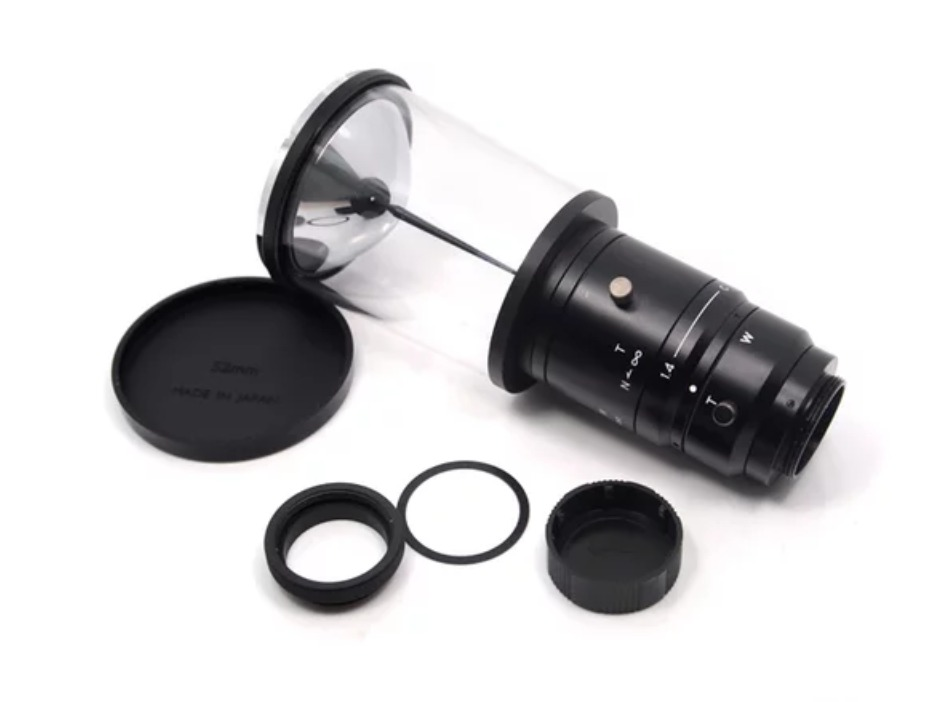
\includegraphics[scale=0.20]{gambar/omnivisino2.jpeg}
  
    % Ubah dengan keterangan gambar yang diinginkan
    \caption{Kamera Omnivsion.}
    \label{fig:omnivision}
\end{figure}
Kamera \emph{omnivision} adalah sebuah kamera yang bisa melihat 360 derajat sekitar 
kamera tersebut \parencite{ref_kamera_omni}. 
Jarak pandang kamera \emph{omnivision} tidak terbatas 
tergantung dari resolusi kamera itu sendiri dan 
konstruksi cerminnya. Pada dasarnya kamera \emph{omnivision} 
adalah kamera biasa yang ditembakkan ke sebuah cermin cembung 
sehingga pandangan kamera tersebut bisa ke segala arah. 

\subsection{Neural Network}
\label{sec:nn}
\begin{figure}[H]
    \centering
  
    % Ubah dengan nama file gambar dan ukuran yang akan digunakan
    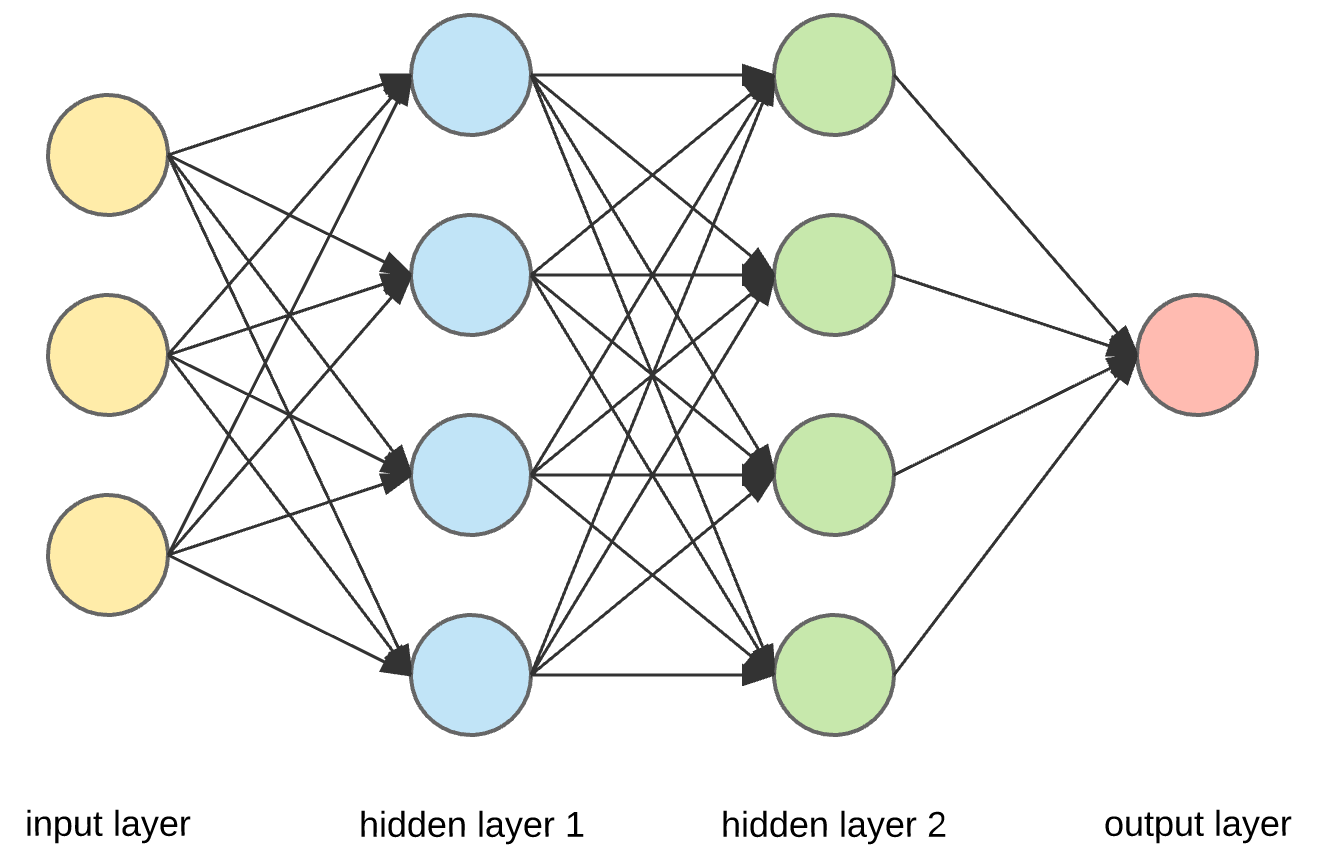
\includegraphics[scale=0.20]{gambar/nn.png}
  
    % Ubah dengan keterangan gambar yang diinginkan
    \caption{Neural Network.}
    \label{fig:nn}
\end{figure}
\emph{Neural network} merupakan bagian dari Pembelajaran Mesin. 
\emph{Neural network} diciptakan untuk mengatasi masalah ketidaklinearan 
pada sebuah model \parencite{ref_neural_network}. Pada dasarnya, 
\emph{Neural network} hanyalah sekumpulan \emph{Neuron} 
yang terhubung oleh sebuah \emph{Weight} dan \emph{Bias}. Selain 
\emph{Weight} dan \emph{Bias}, ada juga namanya \emph{forward propagation} 
menggunakan \emph{activation function} atau 
biasa disebut transfer function. Selain \emph{forward propagation},
 terdapat \emph{backward propagation} menggunakan \emph{loss function}. 

\subsection{\emph{Activation Function}}
\emph{Activation function} adalah sebuah fungsi yang digunakan untuk men-transfer 
data pada masing-masing layer pada \emph{Neural Network}. 
Dalam \emph{Neural Network}, \emph{Activation function} berperan sebagai 
\emph{forward propagation} yaitu perjalanan dari layer input menuju 
layer output. Beberapa \emph{activation Function} memiliki nilai 
saturasi biasanya bernilai 1 contohnya Sigmoid yang bernilai 
pada interval 0 sampai 1. Ada juga \emph{activation Function} lain yaitu 
tanh yang bernilai pada interval -1 sampai 1 \parencite{ref_activation_function}.

\subsection{\emph{Loss Function}}
\emph{loss function} adalah bagian dari \emph{Neural Network} 
yang bertujuan untuk memberikan umpan balik 
pada model tentang baik atau buruknya fase \emph{training}. 
\emph{loss function} pada \emph{Neural Network} bekerja pada jalur 
\emph{Backward Propagation} yaitu dari layer output menuju layer input. 
Ada beberapa macam \emph{loss function} salah satunya adalah MSE 
(\emph{Mean Squared Error}). MSE \emph{loss function} lebih baik digunakan pada 
data dengan nilai fluktuasi yang rendah \Parencite{ref_loss_function}. 

Selain \emph{loss function}, ada sebuah teori lagi yaitu Optimizer. 
Optimizer adalah sebuah algoritma yang bisa digunakan untuk menentukan 
\emph{learning rate} sistem training. \emph{Learning rate} pada 
\emph{Neural Network} digunakan untuk mengatur seberapa cepat model 
akan konvergen terhadap data-datanya. 

\subsection{\emph{Mobile Robot}}
\label{sec:mobile_robot}
\begin{figure}[H]
    \centering
  
    % Ubah dengan nama file gambar dan ukuran yang akan digunakan
    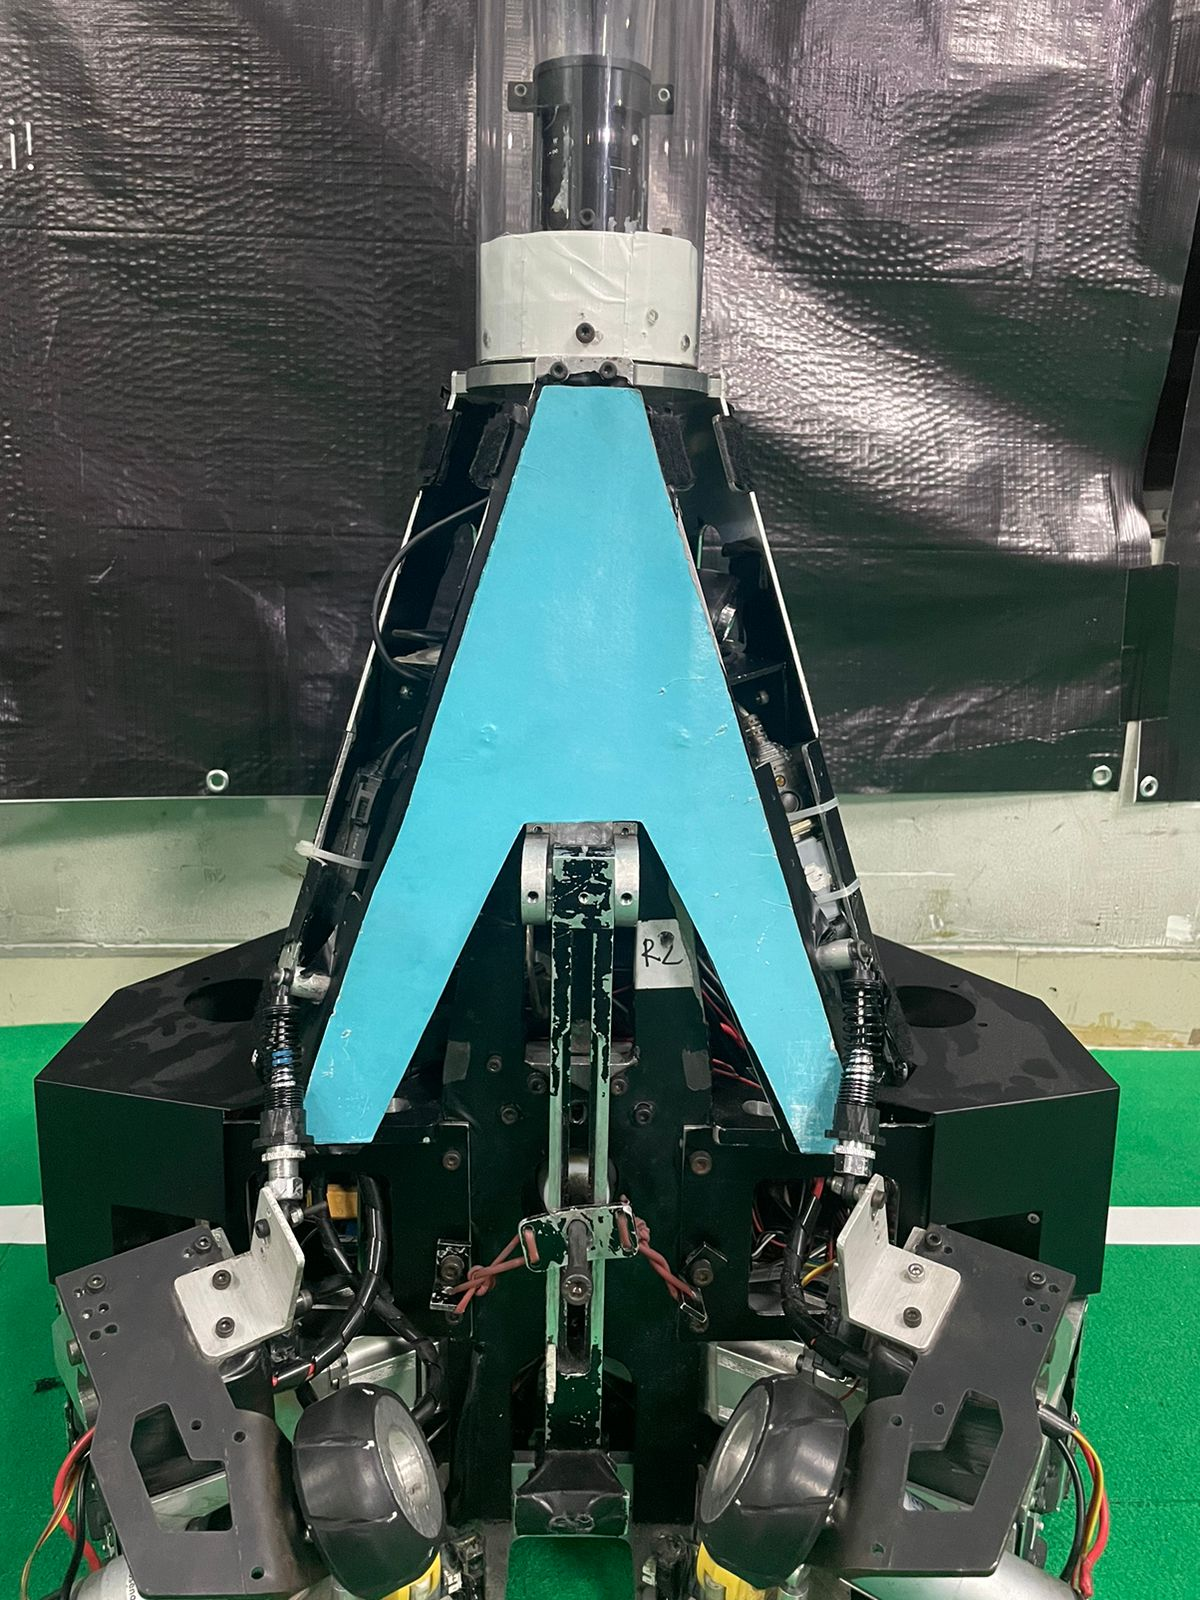
\includegraphics[scale=0.10]{gambar/iris1.jpeg}
  
    % Ubah dengan keterangan gambar yang diinginkan
    \caption{Robot IRIS tampak depan.}
    \label{fig:mobile_robot}
\end{figure}
\emph{Mobile Robot} adalah sebuah robot yang didesain agar bisa bergerak 
atau berpindah tempat dengan mudah. Performa \emph{Mobile Robot} banyak 
dikhususkan pada sistem tracking, lokalisasi, dan algoritma. Ketiga 
hal tersebut berdasar pada kemampuan sensing yang baik \Parencite{ref_mobile_robot}. 
Pada umumnya, sensor yang digunakan adalah kamera baik itu kamera biasa 
maupun kamera \emph{omnivision}. Penggunaan kamera \emph{omnivision} dapat 
membuat robot melihat ke segala arah, Namun pre-processing datanya yang 
lebih sulit dibandingkan dengan kamera biasa.

\subsection{\emph{OpenCV}}
\label{sec:opencv}
\begin{figure}[H]
    \centering
  
    % Ubah dengan nama file gambar dan ukuran yang akan digunakan
    
\includegraphics[scale=0.40]{gambar/opencv.png}
  
    % Ubah dengan keterangan gambar yang diinginkan
    \caption{Logo OpenCV.}
    \label{fig:opencv}
\end{figure}
\emph{OpenCV} adalah library open-source yang dikembangkan oleh 
Intel dengan bahasa pemrograman C/C++. 
\emph{OpenCV} menyediakan banyak algoritma yang berhubungan dengan Visi 
Komputer \Parencite{ref_opencv}. OpenCV banyak digunakan untuk deteksi 
objek baik itu berdasarkan warna, bentuk, ukuran, dan lain lain 
sesuai kebutuhan program. 

\subsection{Robot Operating System}
\label{sec:ros}
\begin{figure}[H]
    \centering
  
    % Ubah dengan nama file gambar dan ukuran yang akan digunakan
    
\includegraphics[scale=0.45]{gambar/ros.png}
  
    % Ubah dengan keterangan gambar yang diinginkan
    \caption{Logo ROS.}
    \label{fig:ros}
\end{figure}
ROS atau \emph{Robot Operating System} adalah sebuah platform yang berdiri 
diatas 
Linux dan berguna untuk sinkronisasi bagian bagian dari 
robot \Parencite{ref_ros}. ROS banyak digunakan sebagai inti 
pemrosesan data dari sebuah robot mulai dari pemrosesan data sensor 
hingga menjadi data aktuator. ROS menyediakan konsep modular programming 
dengan metode publish/subscribe untuk IPC (\emph{Inter Process Communication}) nya. Selain memudahkan untuk 
transfer data antar proses, ROS juga menyediakan timer dengan scheduler 
default nya mengikuti Default Linux Scheduler yaitu Priority-based scheduler. 
Hal itu memungkinkan pengguna untuk mengatur prioritas masing-masing bagian 
dari robotnya. 

\subsection{Websocket}
Websocket adalah jenis protokol komunikasi berbasis protokol TCP (\emph{Transmission Control Protocol}). 
Protokol websocket membuat kedua pengirim dan menerima untuk selalu 
membuka socket nya agar bisa saling komunikasi. 
Dibandingkan dengan HTTP (\emph{Hypertext Transfer Transfer Protocol}), 
protokol Websocket memiliki 
latensi yang lebih baik \Parencite{ref_websocket}. Aplikasi 
websocket banyak digunakan untuk aplikasi obrolan (chat), game online,
 aplikasi yang membutuhkan data \emph{realtime}, dan masih banyak lainnya. 

\cleardoublepage

% Bab 3 desain dan implementasi
\chapter{DESAIN DAN IMPLEMENTASI}
\label{chap:desainimplementasi}

% Ubah bagian-bagian berikut dengan isi dari desain dan implementasi
\section{Deskripsi Sistem}
\label{sec:deskripsisistem}

Sistem terdiri dari empat proses utama yaitu Pengambilan data, \textit{Training} data, Pembuatan \textit{Lookup Table}, dan yang terakhir adalah membaca data dari \textit{Lookup Table} tersebut sehingga menjadi data yang telah terkalibrasi.

\section{Pengambilan Data
  \label{sec:pengambilandata}}

Hal yang dilakukan sebelum pengambilan data adalah menyiapkan robot dan marker yang telah dibuat sebelumnya. Adapun data yang diambil merupakan data koordinat polar baik itu pada kamera maupun pada lapangan. Berikut rumus yang digunakan untuk menghitung koordinat polar pada kamera: 

\begin{equation}
  \begin{aligned}
    dx &= x - x\_center\_cam \\ 
    dy &= y\_center\_cam - y \\
    r &= \sqrt{dx^2 + dy^2} \\
    \theta &= \arctan(\frac{dy}{dx})
  \end{aligned}
\end{equation}

\begin{figure}[H]
  \centering
  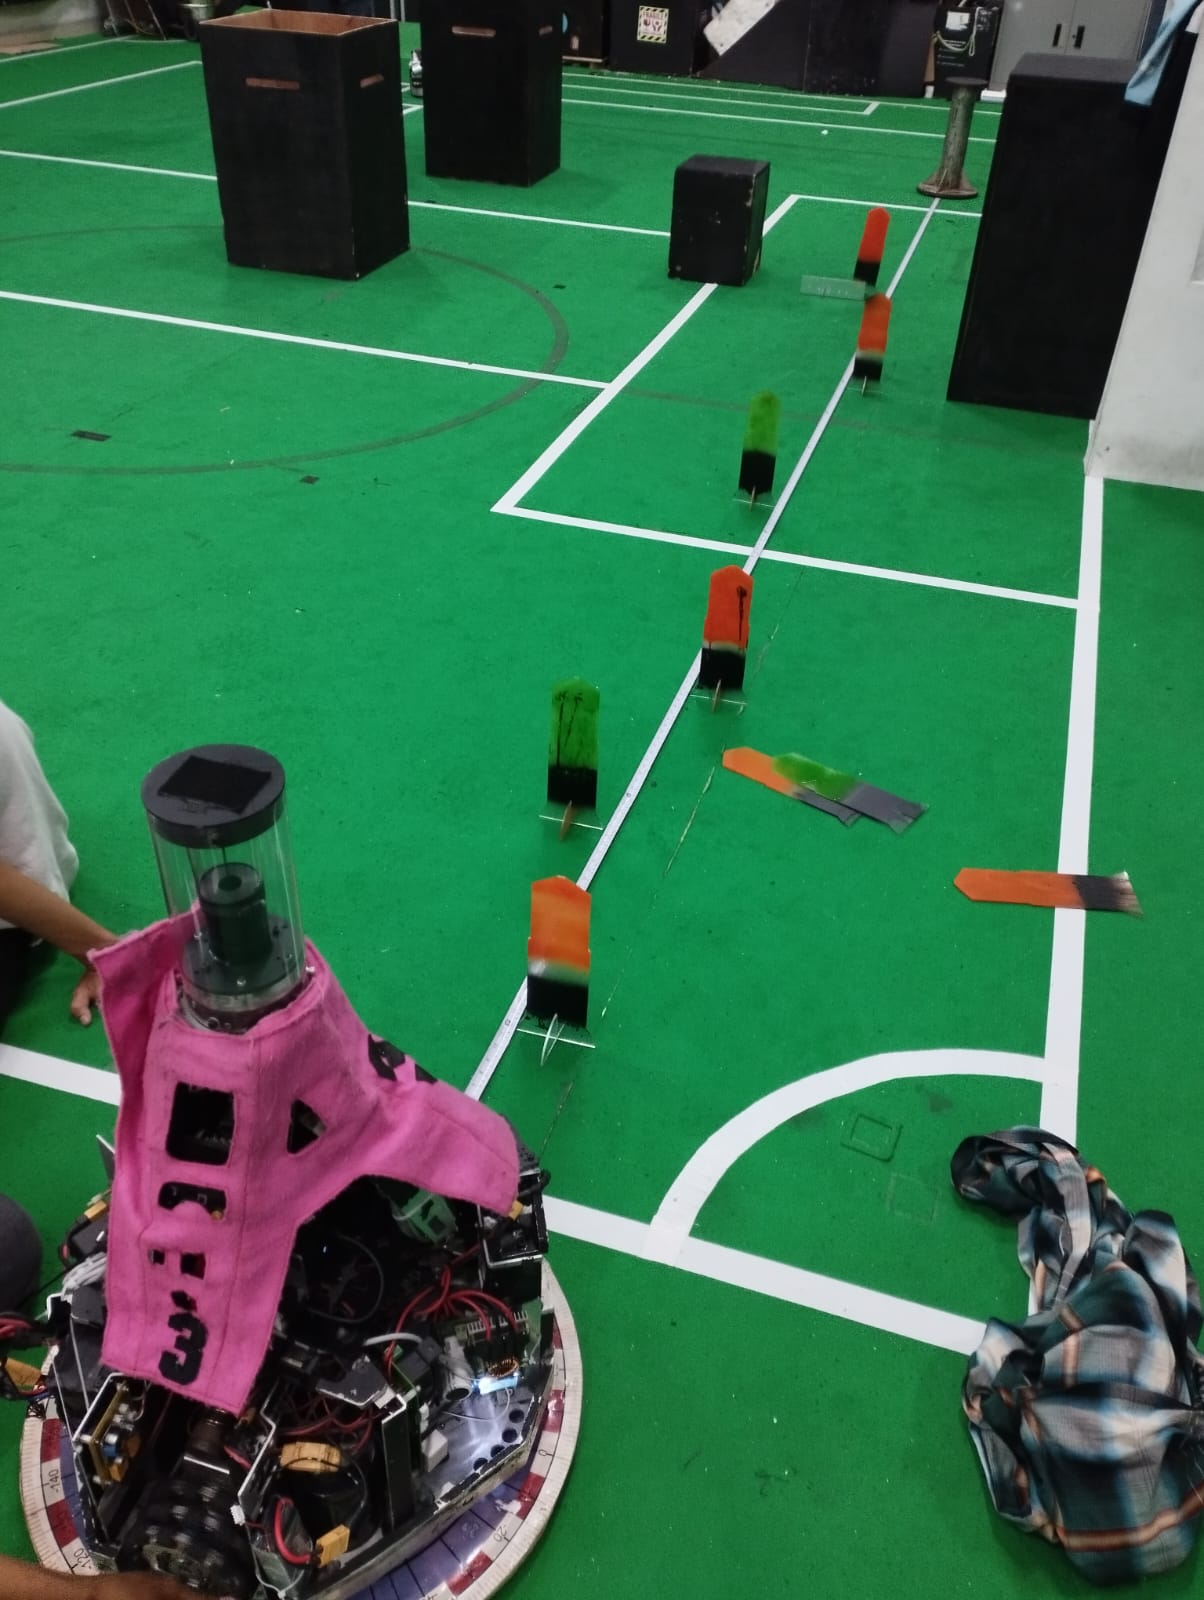
\includegraphics[scale=0.20]{gambar/ambil_data.jpeg}
  \caption{Persiapan robot.}
  \label{fig:persiapanrobot}
\end{figure}

Dikarenakan robot tidak memiliki display, maka untuk mengakses kamera perlu dilakukan dengan mengakses melalui program web yang telah disediakan oleh robot. Berikut adalah program robot untuk mengakses kamera dan mengirim ke web mengunakan \textit{websocket}.

\lstinputlisting[
  language=C++,
  caption={Program akses kamera.},
  label={lst:akseskamera}
]{program/akses_kamera.cpp}

\lstinputlisting[
  language=C++,
  caption={Program publish kamera.},
  label={lst:publishkamera}
]{program/publish_kamera.cpp}

\lstinputlisting[
  language=JavaScript,
  caption={Program akses kamera melalu web.},
  label={lst:kameraweb}
]{program/kamera_web.js}

\begin{figure}[H]
  \centering
  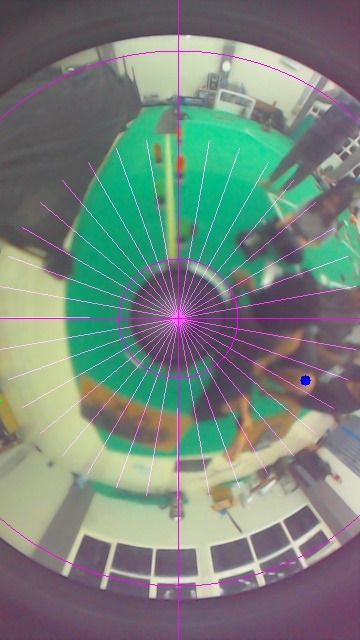
\includegraphics[scale=0.8]{gambar/iris_web.jpeg}
  \caption{Tampilan website robot.}
  \label{fig:webrobot}
\end{figure}

Dari tampilan website tersebut, warna merah pada lapangan bisa diklik dan akan muncul koordinat polar pada kamera. Lalu koordinat-koordinat tersebut akan disimpan ke dalam file. Adapun data yang diambil adalah sebagai berikut:
\begin{figure}[H]
  \centering
  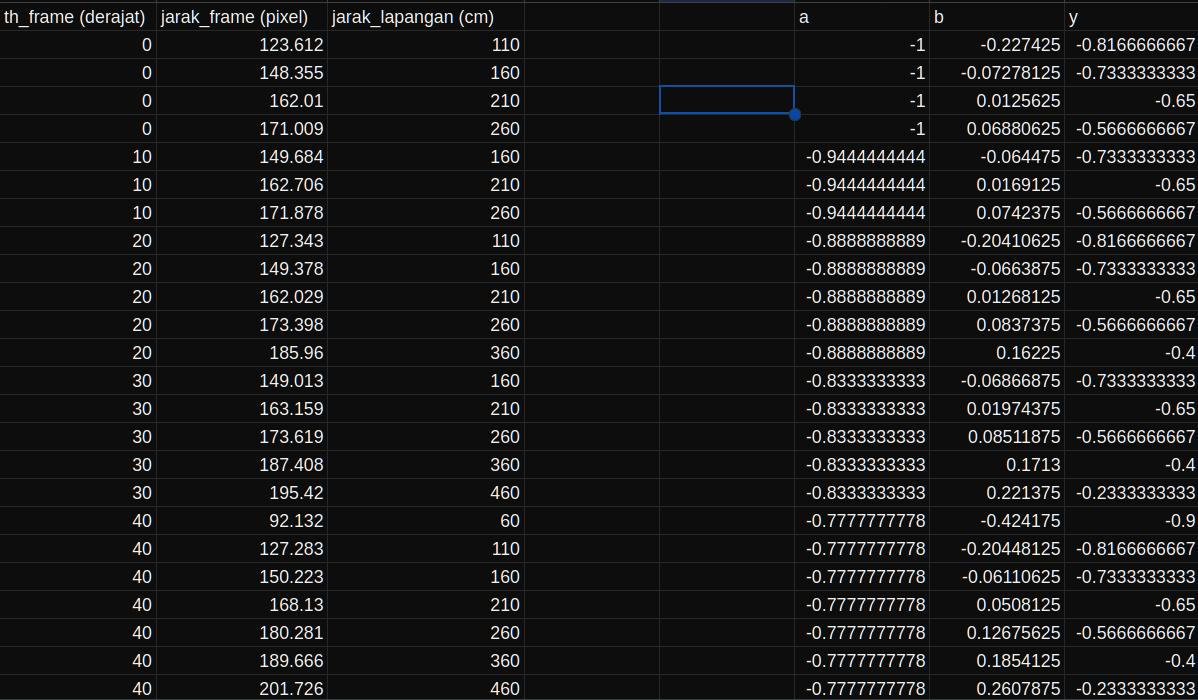
\includegraphics[scale=0.50]{gambar/data.jpg}
  \caption{Data \textit{training}.}
  \label{fig:datatraining}
\end{figure}

\section{\textit{Training} data
  \label{sec:trainingdata}}

Data yang telah diambil kemudian diolah dengan menggunakan program \textit{training} data. Program ini menggunakan metode \textit{Neural Network} untuk mengolah data tersebut. Berikut adalah program \textit{training} data. 

Adapun arsitektur \textit{Neural Network} yang digunakan adalah memiliki 2 \textit{hidden layer} dengan masing-masing 36 dan 36 \textit{neuron}. \textit{Activation function} yang digunakan adalah \textit{Sigmoid} dengan rumusan sebagai berikut: 

\begin{equation}
  \begin{aligned}
    f(x) &= \frac{1}{1 + e^{-x}}
  \end{aligned}
\end{equation}

Keuntungan menggunakan \textit{Sigmoid} adalah karena \textit{Sigmoid} memiliki rentang nilai antara 0 dan 1 yang sesuai dengan data yang akan diolah. 

\textit{Loss function} yang digunakan adalah \textit{Mean Squared Error} dengan rumusan sebagai berikut: 

\begin{equation}
  \begin{aligned}
    L(y, \hat{y}) &= \frac{1}{n} \sum_{i=1}^{n} (y_i - \hat{y_i})^2
  \end{aligned}
\end{equation}

\textit{Optimizer} yang digunakan adalah \textit{Adam} dengan \textit{learning rate} sebesar 0.0001.

Adapun epoch yang digunakan adalah sebanyak 300000 kali. Hal itu bisa berubah tergantung keadaan data yang di-\textit{train}. 

Adapun Arsitektur penuh dari \textit{Neural Network} yang digunakan adalah sebagai berikut: 

\begin{itemize}
    \item \( \mathbf{x} \in \mathbb{R}^2 \): Input data
    \item \( \mathbf{W}^{(1)} \in \mathbb{R}^{36 \times 2} \): weight layer pertama
    \item \( \mathbf{b}^{(1)} \in \mathbb{R}^{36} \): bias layer pertama
    \item \( \mathbf{W}^{(2)} \in \mathbb{R}^{36 \times 36} \): weight layer kedua
    \item \( \mathbf{b}^{(2)} \in \mathbb{R}^{36} \): bias layer kedua
    \item \( \mathbf{W}^{(3)} \in \mathbb{R}^{1 \times 36} \): weight layer ketiga
    \item \( \mathbf{b}^{(3)} \in \mathbb{R}^{1} \): bias layer ketiga
    \item \( \sigma \): sigmoid activation function
\end{itemize}

\begin{equation}
  \textbf{Input ke Hidden Layer Pertama}:
  \begin{aligned}
    \mathbf{z}^{(1)} &= \mathbf{W}^{(1)} \mathbf{x} + \mathbf{b}^{(1)} \\
    \mathbf{a}^{(1)} &= \sigma(\mathbf{z}^{(1)})
  \end{aligned}
\end{equation}

\begin{equation}
  \textbf{Hidden Layer Pertama ke Hidden Layer Kedua}:
  \begin{aligned}
    \mathbf{z}^{(2)} &= \mathbf{W}^{(2)} \mathbf{a}^{(1)} + \mathbf{b}^{(2)} \\
    \mathbf{a}^{(2)} &= \sigma(\mathbf{z}^{(2)})
  \end{aligned}
\end{equation}

\begin{equation}
  \textbf{Hidden Layer Kedua ke Output Layer}:
  \begin{aligned}
    \mathbf{z}^{(3)} &= \mathbf{W}^{(3)} \mathbf{a}^{(2)} + \mathbf{b}^{(3)} \\
    \mathbf{a}^{(3)} &= \mathbf{z}^{(3)}
  \end{aligned}
\end{equation}

% Contoh input potongan kode dari file
\lstinputlisting[
  language=Python,
  caption={Program \textit{train} data.},
  label={lst:traindata}
]{program/train.py}

\section{Pembuatan \textit{Lookup Table}
  \label{sec:pembuatanlut}}

Setelah data di-\textit{train} maka data tersebut akan dijadikan \textit{Lookup Table}. \textit{Lookup Table} ini berisi data-data yang telah di-\textit{train} sebelumnya. Berikut adalah rumusan untuk membuat \textit{Lookup Table} 2 dimensi: 

\begin{equation}
  \begin{aligned}
    size &= \theta\_max \times r\_max \\
    index &= \theta \times r\_max + r
  \end{aligned}
\end{equation}

Dari rumusan tersebut bisa didapat ukuran dari \textit{Lookup Table} yang akan dibuat dan index dari data yang akan dimasukkan ke dalam \textit{Lookup Table}.
Kemudian untuk nilai dari \textit{Lookup Table} itu sendiri berasal dari rumusan \textbf{3.4 - 3.6}.
Adapun program pembuatan \textit{Lookup Table} adalah sebagai berikut.

\lstinputlisting[
  language=Python,
  caption={Program pembuatan \textit{Lookup Table}.},
  label={lst:pembuatanlut}
]{program/save_lut.py}

\section{Pembacaan \textit{Lookup Table}
  \label{sec:pembacaanlut}}

Setelah \textit{Lookup Table} dibuat maka yang terakhir adalah membaca data dari \textit{Lookup Table} dengan rumusan sebagai berikut.  

\begin{equation}
  \begin{aligned}
    index &= \theta\_cam \times r\_max + r\_cam \\
    r\_real &= \textit{Lookup\_Table}[index] \\
    \theta\_real &= \theta\_cam
  \end{aligned}
\end{equation}

Proses tersebut dilakukan pada robot. Berikut adalah program pembacaan \textit{Lookup Table}.

\lstinputlisting[
  language=C++,
  caption={Program membaca \textit{Lookup Table}.},
  label={lst:membacalut}
]{program/read_lut.cpp} 

\cleardoublepage

% Bab 4 pengujian dan analisis
\chapter{PENGUJIAN DAN ANALISIS}
\label{chap:pengujiananalisis}

% Ubah bagian-bagian berikut dengan isi dari pengujian dan analisis

\section{Visualisasi Hasil Kalibrasi}
\label{sec:visualisasihasil} 

Visualisasi hasil kalibrasi dilakukan dengan cara data pada kamera dengan data pada lapangan. Hal itu dilakukan dengan cara memasukkan data pada kamera ke dalam \emph{Lookup Table} yang telah dibuat sebelumnya. Berikut adalah hasil visualisasi yang didapat. 

\begin{figure}[H]
  \centering
  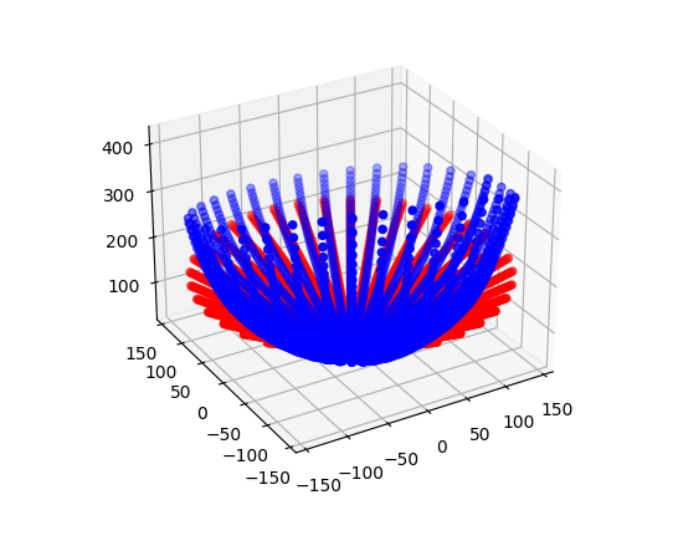
\includegraphics[scale=0.9]{gambar/visual1.png}
  \caption{Visualisasi hasil kalibrasi.}
  \label{fig:hasilkalibrasi}
\end{figure}

Dari gambar tersebut, dapat dilihat bahwa data pada kamera yang digunakan tidak sepenuhnya tegak lurus 90 derajat dengan lapangan. Hal itu terjadi karena kamera yang digunakan tidak terpasang dengan benar. 

\section{Skenario Pengujian Akurasi}
\label{sec:skenariopengujian}

Pengujian dilakukan dengan cara mendeteksi bola yang diam di lapangan dengan memutar robot pada posisinya sendiri. Hal itu membuat robot dapat melihat bola dari berbagai sudut. Pengujian dilakukan dengan mengambil data dari kamera omnivision yang telah terpasang pada robot lalu memroses data tersebut menggunakan \emph{Lookup Table} yang telah dibuat sebelumnya sehingga didapat koordinat bola pada lapangan. Berikut adalah skenario pengujian yang dilakukan: 

\begin{figure}[H]
  \centering
  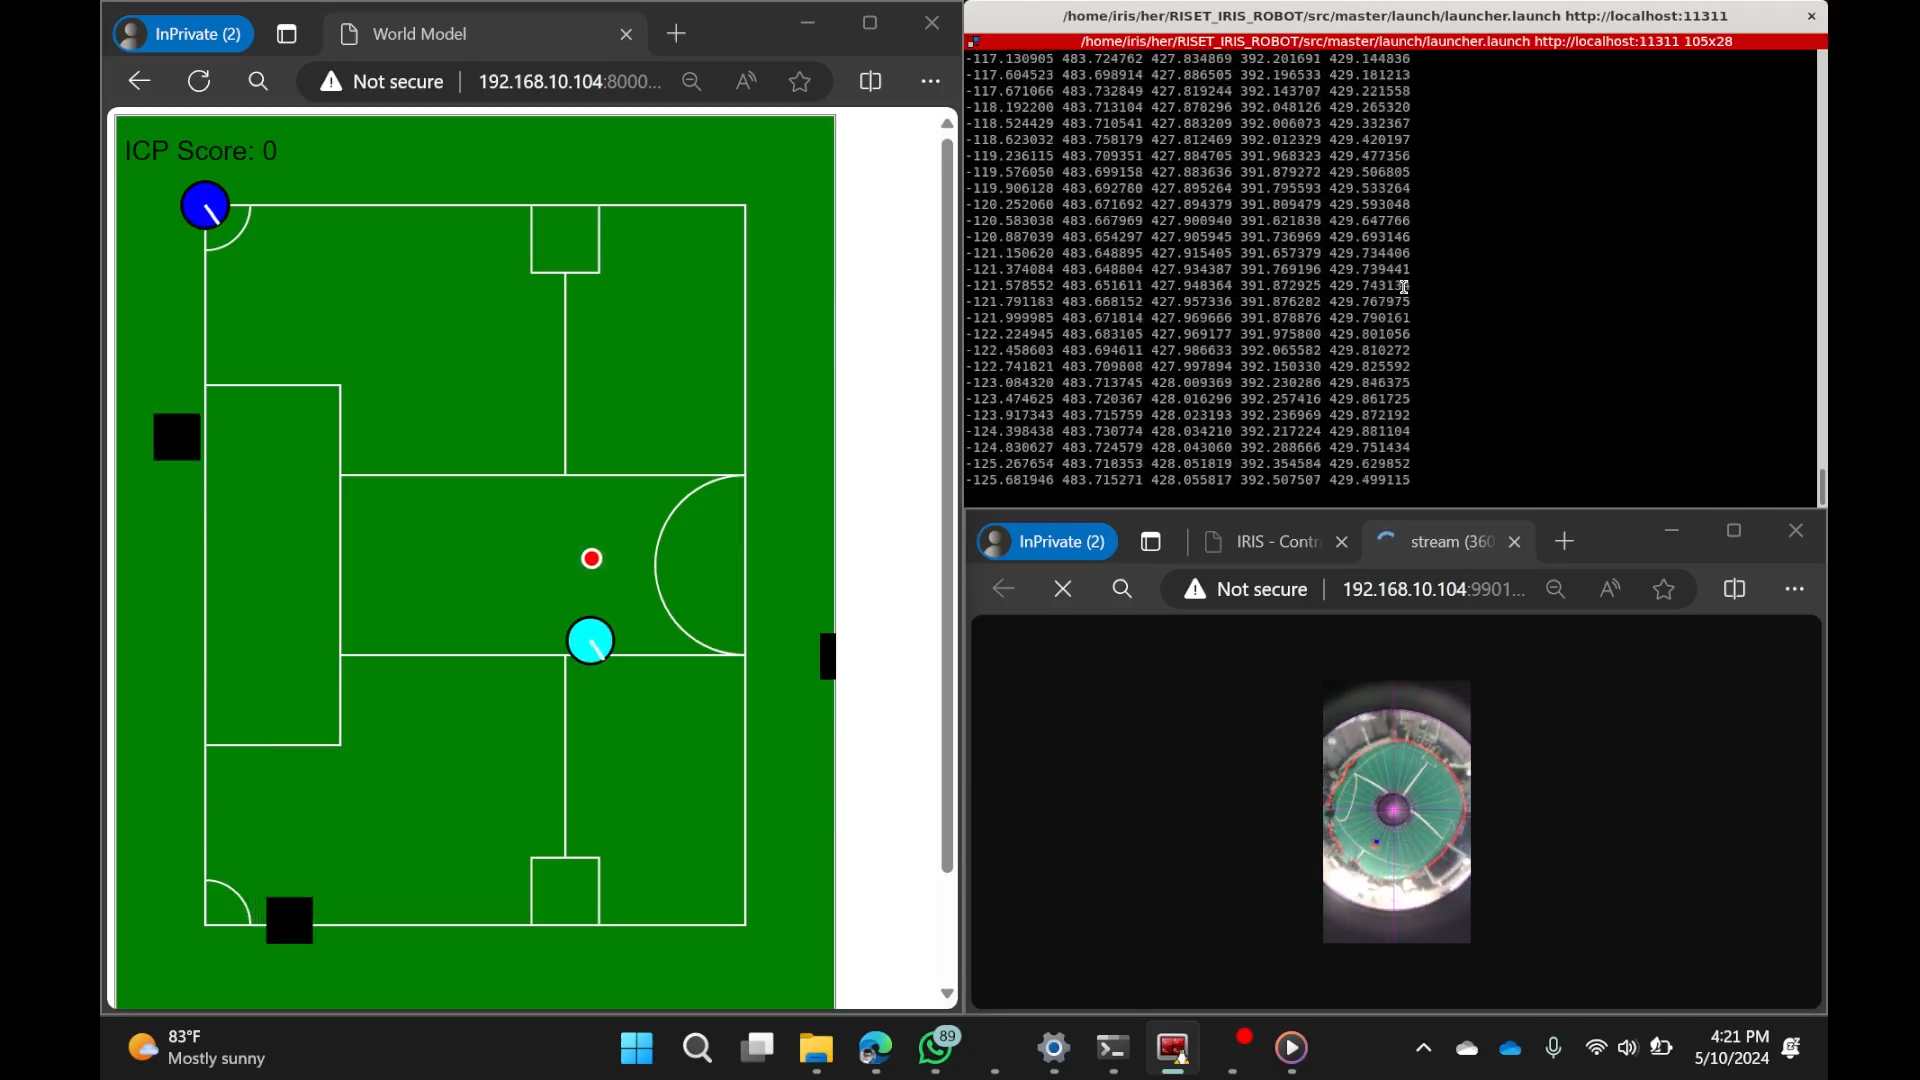
\includegraphics[scale=0.20]{gambar/saat_putar_bola.png}
  \caption{Skenario Pengujian.}
  \label{fig:skenariopengujian}
\end{figure}

Adapun rumusan yang digunakan untuk menghitung posisi bola pada lapangan adalah sebagai berikut: 

\begin{equation}
  \begin{aligned}
    dx &= x\_bola\_cam - x\_center\_cam \\
    dy &= y\_center\_cam - y\_bola\_cam \\
    r\_bola\_cam &= \sqrt{dx^2 + dy^2} \\
    \theta\_bola\_cam &= \arctan(\frac{dy}{dx}) \\
    index &= \theta\_bola\_cam \times r\_max + r\_bola\_cam \\ 
    r\_bola\_lap &= r\_lookup[index] \\
    \theta\_bola\_lap &= \theta\_bola\_cam + robot\_pose\_\theta - 90 \\
    x\_bola &= robot\_pose\_x + r\_bola\_lap \times \cos(\theta\_bola\_lap) \\
    y\_bola &= robot\_pose\_y + r\_bola\_lap \times \sin(\theta\_bola\_lap) \\
  \end{aligned}
\end{equation}

\section{Evaluasi Pengujian Akurasi}
\label{sec:analisispengujian}

Dari pengujian yang telah dilakukan, didapat data sebagai berikut:

% Contoh pembuatan tabel
\begin{longtable}{|c|c|c|}
  \caption{Hasil Pengujian Posisi Bola pada Lapangan}
  \label{tb:posisibolalapangan}                                   \\
  \hline
  \rowcolor[HTML]{C0C0C0}
  \textbf{Sudut Robot ke Bola} & \textbf{Posisi Bola X} & \textbf{Posisi Bola Y} \\
  \hline
  0 deg            & 380.14 cm                & 420.93 cm            \\
  30 deg           & 386.72 cm                & 420.77 cm            \\
  60 deg           & 387.15 cm                & 420.94 cm            \\
  90 deg           & 387.70 cm                & 421.69 cm           \\
  120 deg           & 386.97 cm                & 431.32 cm           \\
  150 deg           & 389.73 cm                & 431.77 cm           \\
  180 deg           & 389.71 cm                & 430.90 cm           \\
  210 deg           & 392.98 cm                & 430.02 cm           \\
  240 deg           & 391.82 cm                & 429.64 cm           \\
  270 deg           & 388.43 cm                & 426.11 cm           \\
  300 deg           & 386.68 cm                & 424.20 cm           \\
  330 deg           & 385.83 cm                & 421.27 cm           \\
  \hline
\end{longtable}

Dari tabel tersebut didapat standar deviasi pada sumbu x sebesar 2.83 cm sedangkan pada sumbu y sebesar 5.71 cm. Hal itu menunjukkan bahwa hasil pengujian yang dilakukan cukup akurat. 

\section{Skenario Pengujian Akurasi Kedua}
\label{sec:skenariopengujian}

Pengujian akurasi kedua adalah dengan cara robot mendeteksi garis dan membuat visualisasi dari garis tersebut. Pengujian dilakukan dengan cara robot diletakkan di daerah lapangan yang dekat dengan garis dan robot akan melihat sekelilingnya.  

\begin{figure}[H]
  \centering
  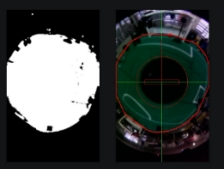
\includegraphics[scale=1.2]{gambar/cam_raw1.jpg}
  \caption{Skenario Pengujian Akurasi Kedua.}
  \label{fig:skenariopengujian}
\end{figure}

Gambar disebelah kiri adalah hasil dari deteksi lapangan yang nantinya akan digunakan untuk mendeteksi garis. Sedangkan gambar disebelah kanan adalah gambar \textit{bgr} dari kamera omnivision. 

\section{Evaluasi Pengujian Akurasi Kedua}
\label{sec:analisispengujian}

Untuk mendapatkan data garis pada lapangan yang telah terdeteksi, maka data tersebut harus dikalkulasi terlebih dahulu. 

\begin{equation}
  \begin{aligned}
    \textbf{Untuk setiap titik pada hasil deteksi garis:} \\
    dx &= x\_titik[i] - x\_center\_cam \\
    dy &= y\_center\_cam - y\_titik[i] \\
    r\_garis\_pcl\_cam &= \sqrt{dx^2 + dy^2} \\
    \theta\_garis\_pcl\_cam &= \arctan(\frac{dy}{dx}) \\
    index &= \theta\_garis\_pcl\_cam \times r\_max + r\_garis\_pcl\_cam \\ 
    r\_garis\_pcl\_lap &= r\_lookup[index] \\
    \theta\_garis\_pcl\_lap &= \theta\_garis\_pcl\_cam + robot\_pose\_\theta - 90 \\
    x\_garis\_pcl[i] &= robot\_pose\_x + r\_garis\_pcl\_lap \times \cos(\theta\_garis\_pcl\_lap) \\
    y\_garis\_pcl[i] &= robot\_pose\_y + r\_garis\_pcl\_lap \times \sin(\theta\_garis\_pcl\_lap) \\
  \end{aligned}
\end{equation}

Dari kalkulasi yang telah dilakukan, didapat data gambar sebagai berikut:

\begin{figure}[H]
  \centering
  
\includegraphics[scale=1.2]{gambar/cam_raw2.jpg}
  \caption{Hasil Pengujian Akurasi Kedua.}
  \label{fig:hasilpengujian}
\end{figure}

Gambar disebelah kiri adalah hasil dari deteksi garis yang dilakukan oleh robot. Hasil garis tersebut merupakan hasil yang sudah diolah dengan hasil deteksi lapangan. Garis tersebut adalah garis yang belum dikalibrasi. Sedangkan gambar disebelah kanan adalah hasil dari garis yang sudah dikalibrasi. 

\section{Skenario Pengujian Kecepatan Komputasi}
\label{sec:analisispengujian}

Pengujian dilkukan dengan cara membandingkan apakah sistem kalibrasi baru lebih cepat dibandingkan menggunakan sistem kalibrasi lama. Pada robot, sistem kalibrasi baru hanya menggunakan sebuah \emph{Lookup Table} yang berisi data kalibrasi kamera, Sedangkan sistem kalibrasi lama menggunakan algoritma \emph{regresi polynomial}. Berikut adalah source code yang digunakan untuk menghitung waktu komputasi dari kedua sistem kalibrasi tersebut: 

\lstinputlisting[
  language=C++,
  caption={Program Uji waktu.},
  label={lst:ujiwaktu}
]{program/test_waktu.cpp}

\section{Evaluasi Pengujian Kecepatan Komputasi}
\label{sec:analisispengujian}

Dari pengujian yang telah dilakukan, didapat data sebagai berikut: 
\begin{figure}[H]
  \centering
  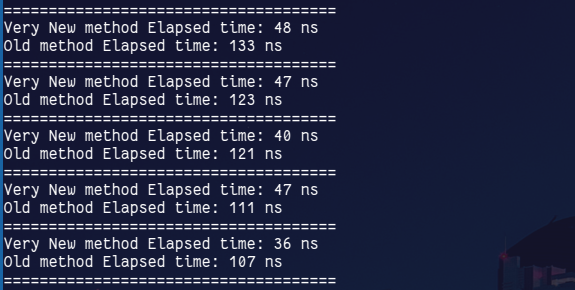
\includegraphics[scale=0.9]{gambar/beda_waktu.png}
  \caption{Evaluasi pengujian waktu.}
  \label{fig:ujiwaktu}
\end{figure}

Dari grafik tersebut dapat dilihat bahwa sistem kalibrasi baru lebih cepat 75.4 ns dibandingkan dengan sistem kalibrasi lama. Dengan rata-rata Kalibrasi baru membutuhkan waktu 43.6 ns sedangkan kalibrasi lama membutuhkan waktu 119 ns. 

\cleardoublepage

% Bab 5 penutup
\chapter{PENUTUP}
\label{chap:penutup}

% Ubah bagian-bagian berikut dengan isi dari penutup

\section{Kesimpulan}
\label{sec:kesimpulan}

Berdasarkan hasil penelitian yang telah dilakukan, maka dapat diambil beberapa kesimpulan sebagai berikut:

\begin{enumerate}[nolistsep]

  \item Dengan melakukan pendekatan non-linear menggunakan Machine Learning untuk kalibrasi kamera, maka hasil kalibrasi kamera lebih baik dibandingkan dengan menggunakan regresi polynomial sederhana.

  \item Sistem kalibrasi dapat meng-kalibrasi semua arah pada kamera omnivision tanpa perlu instalasi ulang hardware jika ada masalah.

\end{enumerate}

\section{Saran}
\label{chap:saran}


Untuk pengembangan lebih lanjut pada penelitian ini, bisa dilakukan beberapa hal antara lain:

\begin{enumerate}[nolistsep]

  \item Mempercepat proses pengambilan data.

  \item Memperbaiki pola pengambilan data sehingga didapat data-data yang lebih baik untuk dilakukan proses \textit{Machine Learning}.
\end{enumerate}


\cleardoublepage

\chapter*{DAFTAR PUSTAKA}
\addcontentsline{toc}{chapter}{DAFTAR PUSTAKA}
\renewcommand\refname{}
\vspace{2ex}
\renewcommand{\bibname}{}
\begingroup
\def\chapter*#1{}
\printbibliography
\endgroup
\cleardoublepage

% Biografi penulis
\begin{center}
  \Large
  \textbf{BIOGRAFI PENULIS}
\end{center}

\addcontentsline{toc}{chapter}{BIOGRAFI PENULIS}

\vspace{2ex}

\begin{wrapfigure}{L}{0.3\textwidth}
  \centering
  \vspace{-3ex}
  % Ubah file gambar berikut dengan file foto dari mahasiswa
  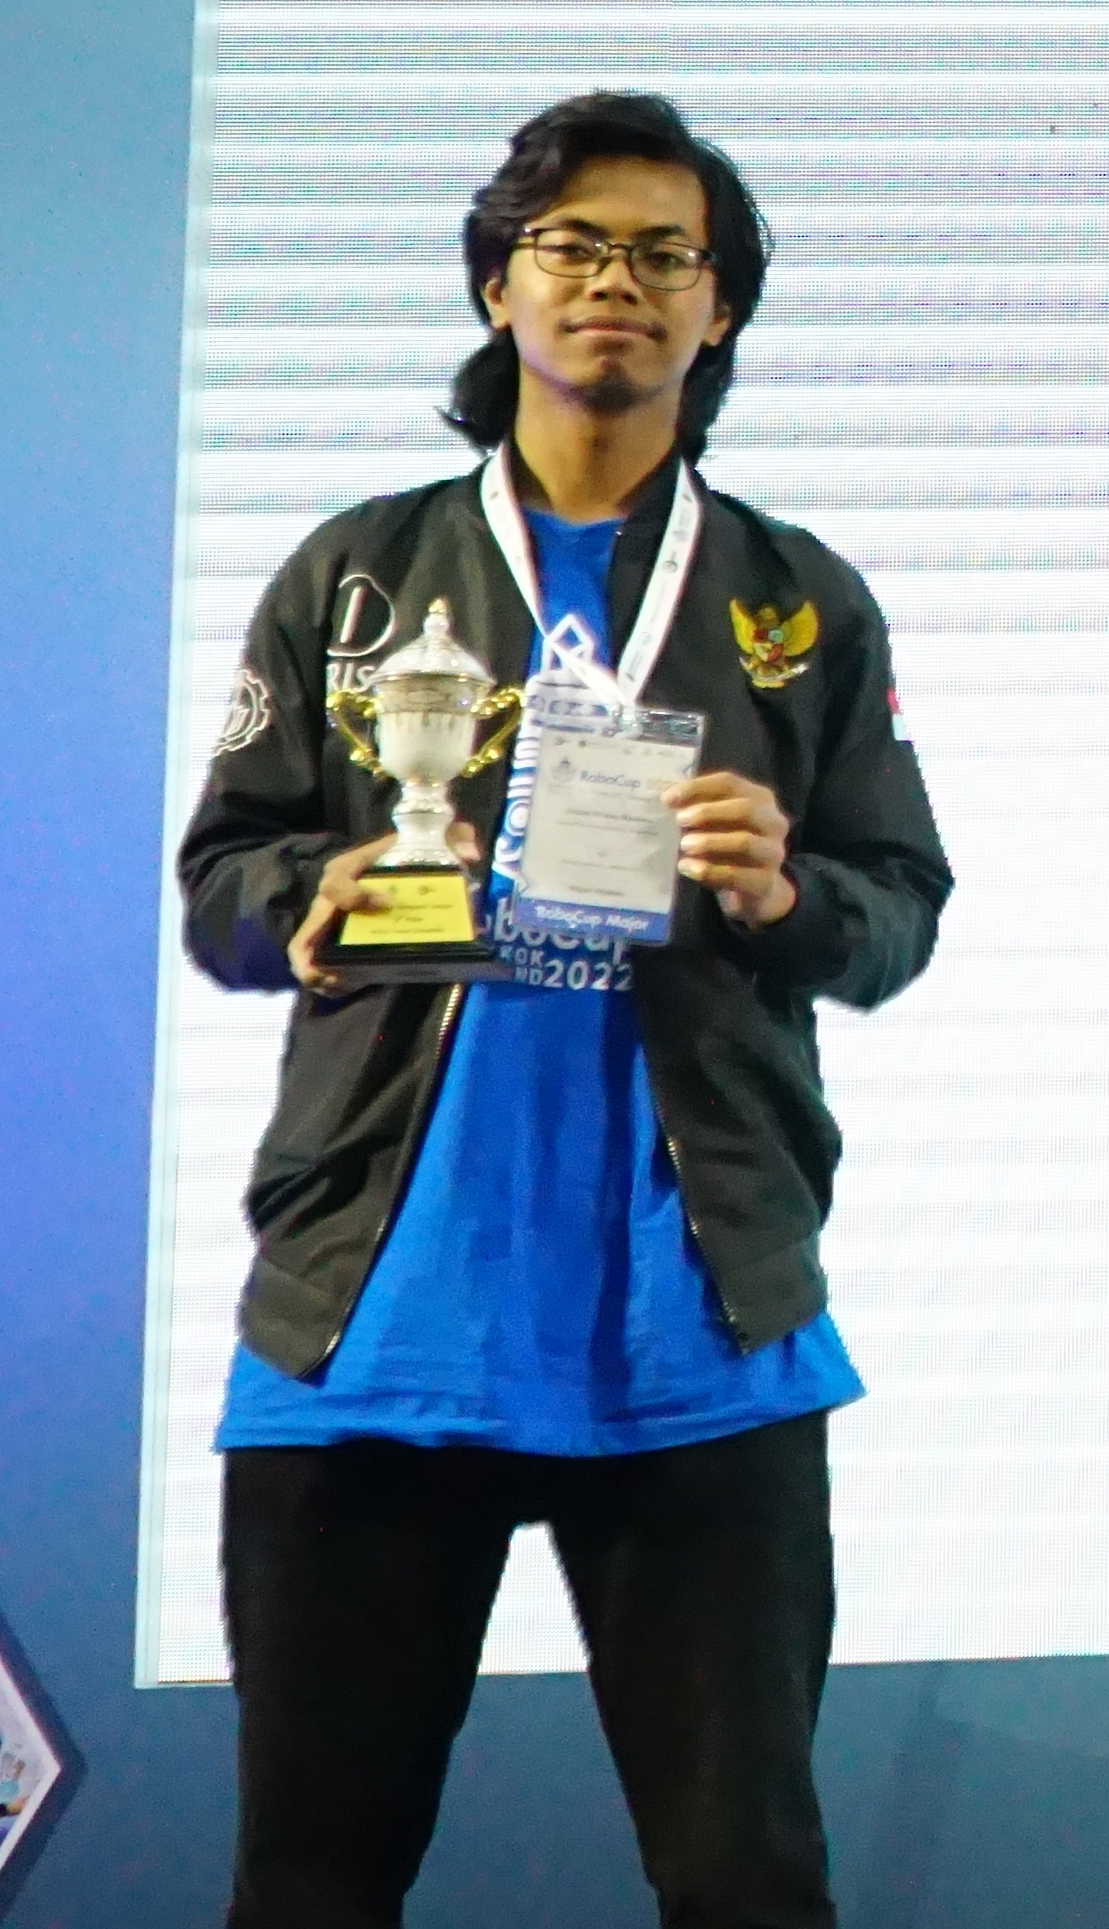
\includegraphics[width=0.3\textwidth]{gambar/foto_piala_asli_cropped.jpg}
  \vspace{-4ex}
\end{wrapfigure}

% Ubah kalimat berikut dengan biografi dari mahasiswa
\name{}, lahir pada 4 Juni 2002, di Jember. Penulis merupakan mahasiswa Program Studi Teknik Komputer angkatan 2020. Penulis merupakan mahasiswa yang aktif dalam kegiatan organisasi dan kegiatan kemahasiswaan. Penulis juga aktif dalam kegiatan penelitian dan pengembangan teknologi. Penulis memiliki ketertarikan dalam bidang pengembangan teknologi dan kecerdasan buatan. Penulis juga aktif dalam kegiatan kompetisi robotika dan berhasil meraih juara 3 dalam kompetisi RoboCup 2022. Penulis juga aktif dalam kegiatan penelitian dan pengembangan teknologi. Penulis memiliki ketertarikan dalam bidang pengembangan teknologi dan kecerdasan buatan. Penulis juga aktif dalam kegiatan kompetisi robotika dan berhasil meraih juara 3 dalam kompetisi RoboCup 2022.

\cleardoublepage

\end{document}
